\section{Sistemas Tolerantes a Fallas}

% ==============================================
\begin{frame}{Confiabilidad}
	\begin{block}{Confiabilidad}
    	Probabilidad de que un sistema pueda cumplir con su función de manera correcta en un intervalo de tiempo $\left[t_0;t\right]$, dado que sí podía hacerlo en $t_0$.
    \end{block}
    \begin{itemize}
    	\item $R$(t) = $\mathbb{P}$(no ocurra ninguna falla en $[t_0;t]$)
    	\item Incrementar esta probabilidad equivale a incrementar la confiabilidad.
    	\item Se busca \textbf{evitar} la ocurrencia de fallas en el sistema.
    	\item Esto tiene algunos incovenientes:
    	\begin{enumerate}
    		\item Uso de componentes que pueden ser muy costosos.
    		\item Dificultades en la etapa de diseño del sistema.
    		\item Errores de diseño no tenidos en cuenta pueden llegar a causar fallas.
    	\end{enumerate}
	\end{itemize}
\end{frame}

% ==============================================
\begin{frame}{Tolerancia a Fallas}
	\begin{itemize}
		\item Una decisión más conservadora consiste en \textbf{tolerar} fallas.
	\end{itemize}
	\begin{block}{Sistema Tolerante a Fallas}
    	No es aquel donde no ocurren fallas. Al contrario, se acepta que las fallas pueden ocurrir. En consecuencia, incluyen mecanismos para que, a pesar de la ocurrencia de una falla, el sistema pueda seguir cumpliendo su función.
    \end{block}
    \begin{itemize}
    	\item Una de las técnicas más comunes es el uso de \textbf{redundancias}.
    	\item Esta consiste en el uso de varias réplicas que realicen las mismas tareas dentro del sistema.
    	\item Por ejemplo, sensores, actuadores, computadoras de vuelo, etc.
    \end{itemize}
\end{frame}

% ==============================================
\begin{frame}{Tolerancia a Fallas: Avión}
	\begin{center}
		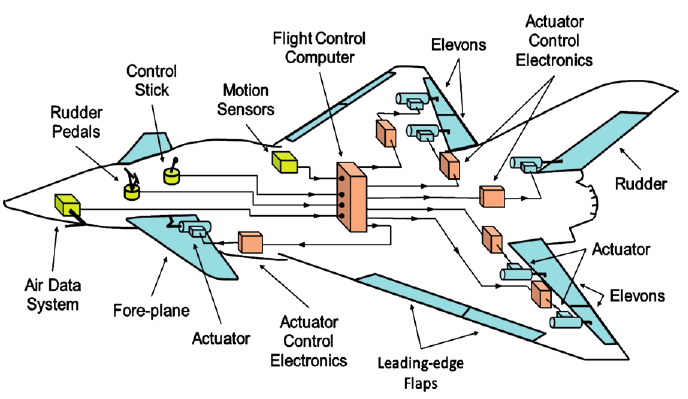
\includegraphics[width=0.7\textwidth]{img/avion_FBW.png}
	\end{center}
	\begin{itemize}
		\item Sensores x4
		\item Actuadores x4
		\item Computadora de vuelo x4
	\end{itemize}
\end{frame}

\begin{frame}{Tolerancia a Fallas: Avión}
	\begin{columns}
		\column{0.5\textwidth}
			\begin{itemize}
				\item <3->\textbf{Todas} las computadoras de vuelo adquieren datos de \textbf{todos} los sensores redundantes.
				\item <4->A partir de la \textbf{comparación de valores}, se detectan fallas de los sensores.
				\item <5->Para tolerar la falla, cada computadora de vuelo selecciona \textbf{un único valor}.
				\item <6->Para ello hay un intercambio entre las 4 computadoras de vuelo.
			\end{itemize}
		\column{0.5\textwidth}
			\begin{overprint}
				\onslide<2>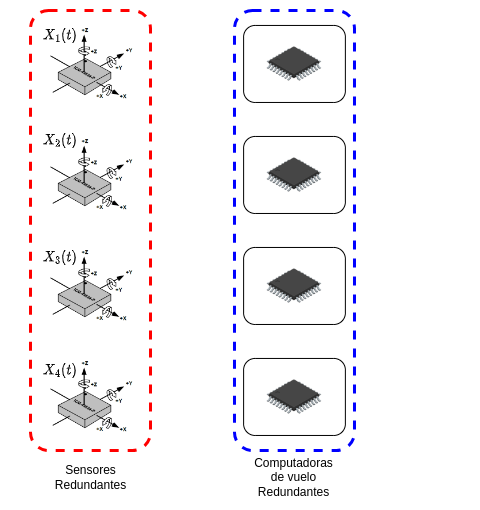
\includegraphics[width=\textwidth]{img/adquieren_sensores_1.png}
				\onslide<3>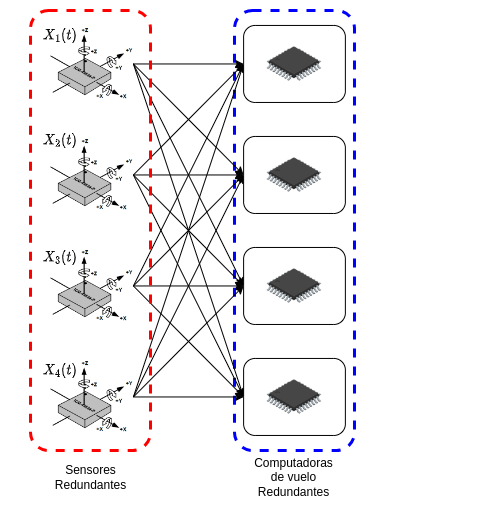
\includegraphics[width=\textwidth]{img/adquieren_sensores_2.png}
				\onslide<4>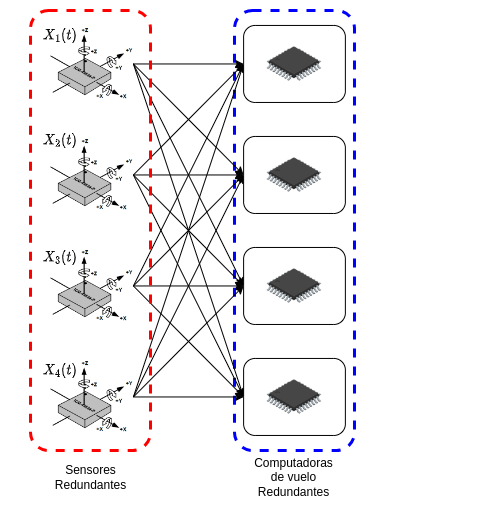
\includegraphics[width=\textwidth]{img/adquieren_sensores_2.png}
				\onslide<5>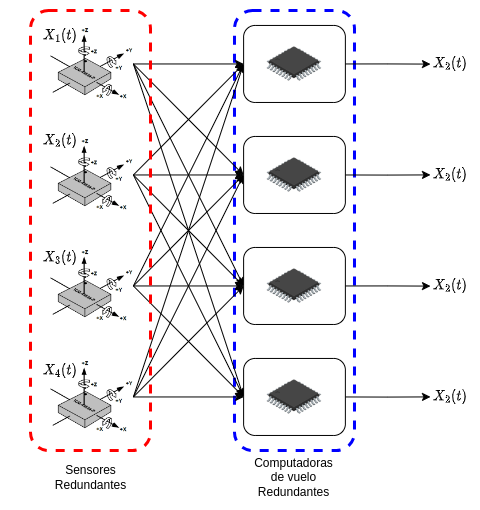
\includegraphics[width=\textwidth]{img/adquieren_sensores_3.png}
				\onslide<6>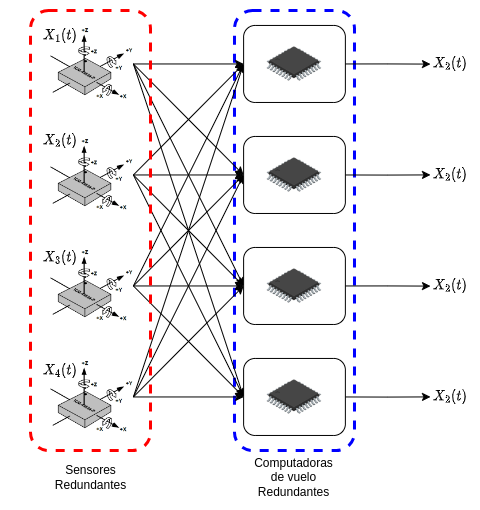
\includegraphics[width=\textwidth]{img/adquieren_sensores_3.png}
			\end{overprint}
	\end{columns}
\end{frame}

\begin{frame}{Tolerancia a Fallas: Avión}
	\begin{columns}
		\column{0.5\textwidth}
			\begin{itemize}
				\item <2->Se calcula la señal a aplicar a los actuadores.
				\item <3->Se realiza un nuevo intercambio para tolerar fallas de las computadoras de vuelo.
				\item <4->Se decide por \textbf{un único valor} de señal $Y(t)$.
				\item <5->Se aplica la señal a los actuadores.
			\end{itemize}
		\column{0.5\textwidth}
			\begin{overprint}
				\onslide<1>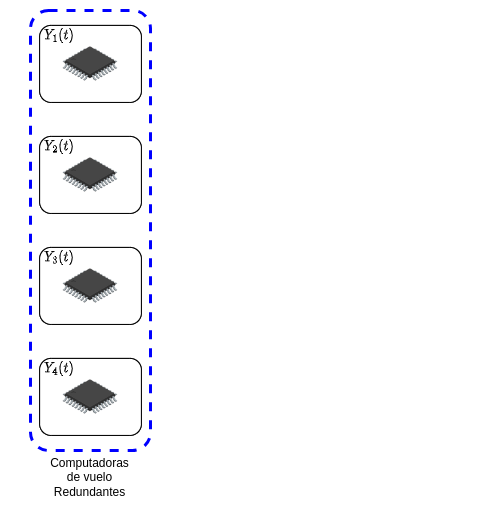
\includegraphics[width=\textwidth]{img/calculo_actuacion_1.png}
				\onslide<2>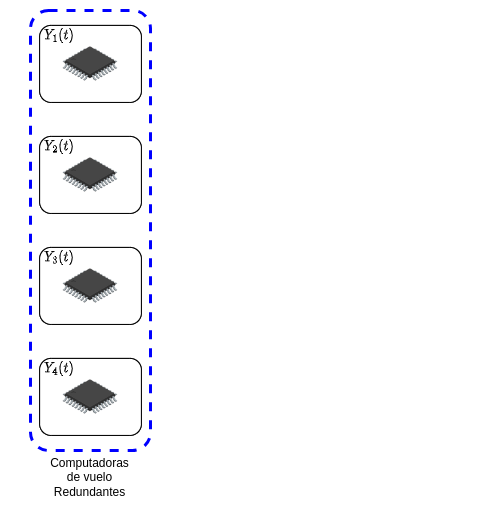
\includegraphics[width=\textwidth]{img/calculo_actuacion_1.png}
				\onslide<3>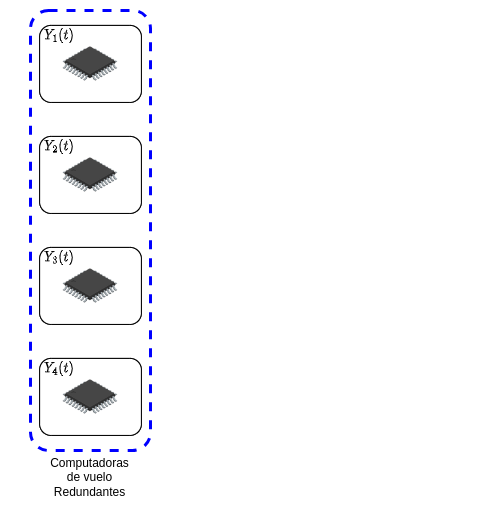
\includegraphics[width=\textwidth]{img/calculo_actuacion_1.png}
				\onslide<4>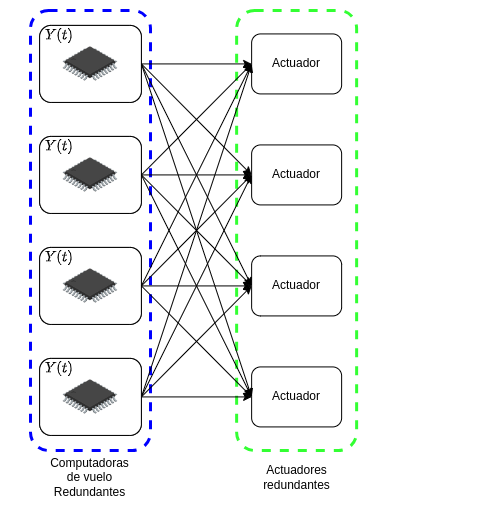
\includegraphics[width=\textwidth]{img/calculo_actuacion_2.png}
				\onslide<5>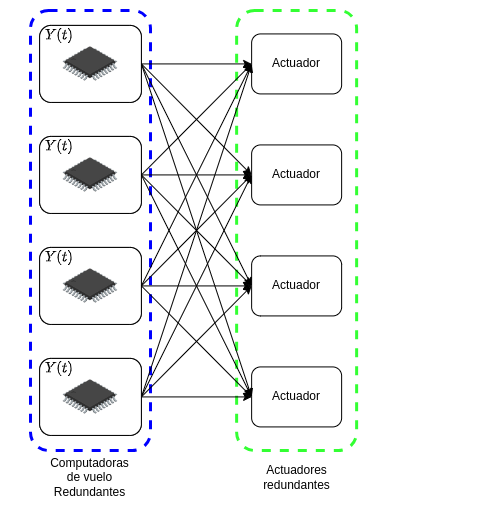
\includegraphics[width=\textwidth]{img/calculo_actuacion_2.png}
			\end{overprint}
	\end{columns}
\end{frame}

\begin{frame}{Tolerancia a Fallas: Avión}
	\begin{center}
		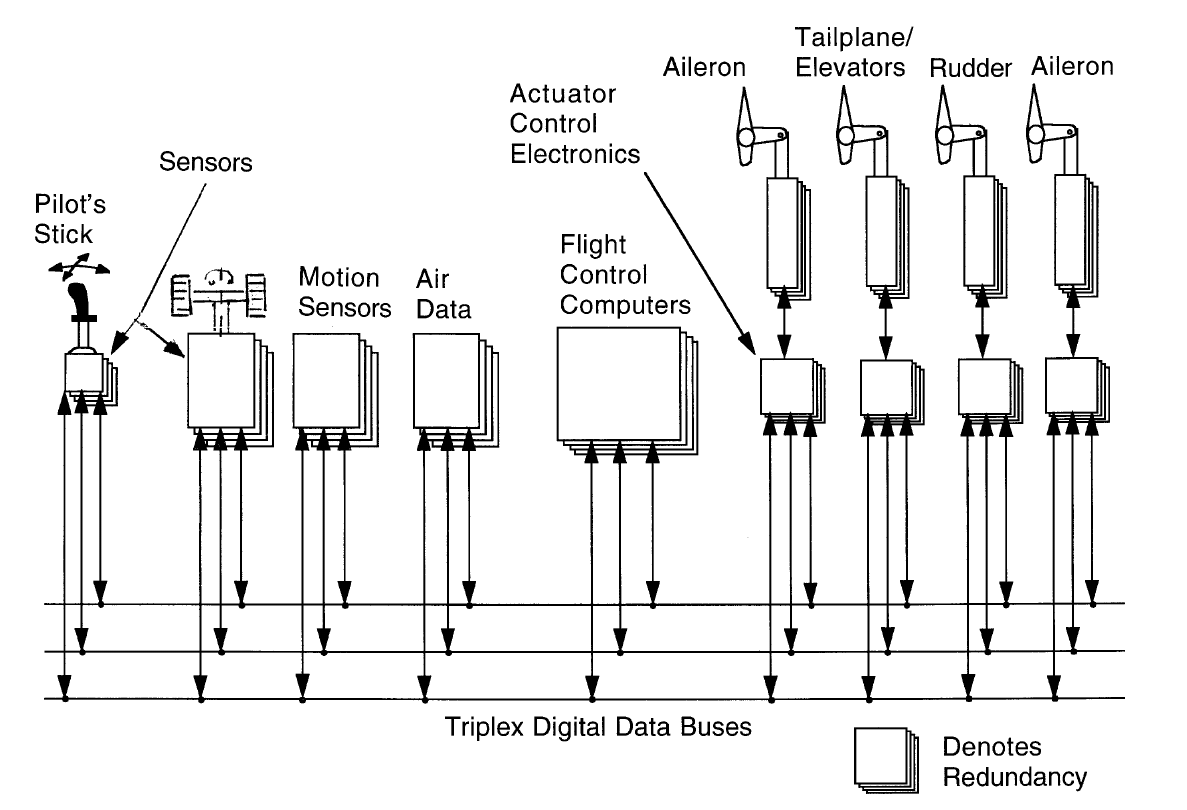
\includegraphics[width=0.68\textwidth]{img/diagrama_general_fly_by_wire.png}
	\end{center}
	\begin{itemize}
		\item Se utiliza un \textbf{bus de comunicaciones} redundante.
		\item Acceso al medio por turnos: \textit{time-division multiple access.}
	\end{itemize}
\end{frame}

% ==============================================
\begin{frame}{Tolerancia a Fallas: Drones}
	\begin{itemize}
		\item Existen algunas computadoras de vuelo comerciales que ofrecen la posibilidad de trabajar con redundancias.
		\item Sin embargo sus costos son muy elevados.
		\item Pueden encontrarse varios trabajos de computadoras de vuelo redundantes que utilizan componentes económicos y accesibles.
		\item Los trabajos que se tomaron como referencia utilizan configuraciones variadas: redundancia doble, triple y cuádruple.
		\item Se mencionan las características comunes.
	\end{itemize}
\end{frame}

\begin{frame}{Tolerancia a Fallas: Redundancia Doble}
	\begin{columns}
		\column{0.6\textwidth}
			\begin{itemize}
				\item Configuración Simple.
				\item La comparación permite detectar si ocurrió una falla o no.
				\item Pero \textbf{no se puede saber cuál de ellas lo hizo!}
				\item Cada réplica debería ejecutar una rutina para detectar la falla.
				\item Esto puede perjudicar el determinismo temporal del sistema de control.
			\end{itemize}
		\column{0.4\textwidth}
			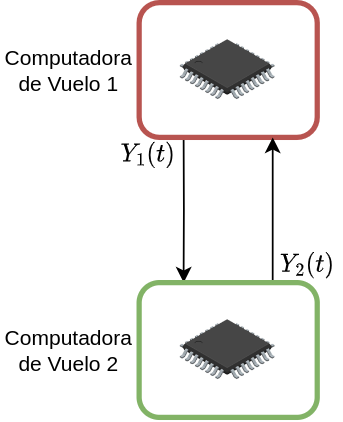
\includegraphics[width=0.8\textwidth]{img/redundancia_doble.png}
	\end{columns}
\end{frame}

\begin{frame}{Tolerancia a Fallas: Redundancia Triple}
	\begin{itemize}
		\item Se asume que una sola de ellas fallará de forma simultánea.
		\item La comparación sí permite detectar cuál falló: 2 de 3.
		\item Punto Singular de Falla: ¿Qué sucede si falla el Árbitro?
		\item Este debe ser altamente confiable, volviéndolo muy costoso.
	\end{itemize}
	\begin{center}
		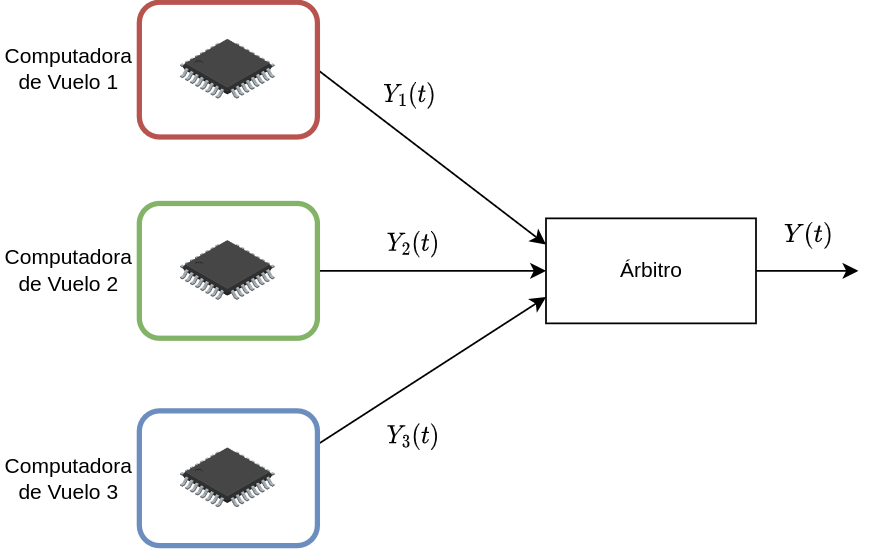
\includegraphics[width=0.6\textwidth]{img/redundancia_triple.png}
	\end{center}
\end{frame}

\begin{frame}{Tolerancia a Fallas: Redundancia Triple}
	\begin{itemize}
		\item Puede eliminarse el árbitro utilizando la siguiente configuración.
		\item Esta configuración es como la del caso del avión.
	\end{itemize}
	\begin{center}
		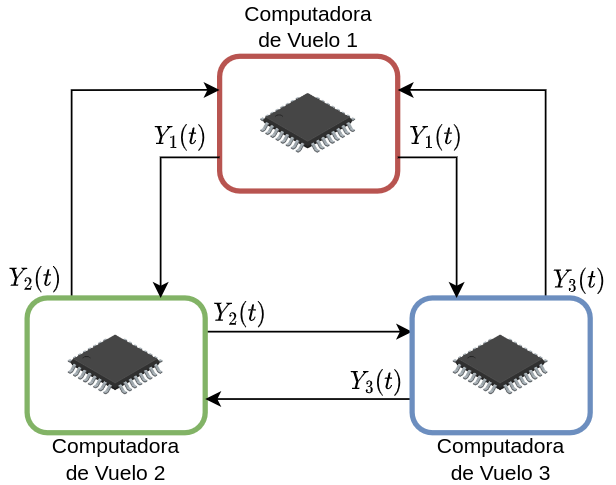
\includegraphics[width=0.6\textwidth]{img/redundancia_triple_sin_arbitro.png}
	\end{center}
\end{frame}

\begin{frame}{Problema del Consenso}
	\begin{itemize}
		\item Si todas las réplicas utilizan los mismos valores de entrada.
		\item Entonces llegan a la misma conclusión acerca del valor seleccionado.
		\item Que pasa si...
	\end{itemize}
	\begin{columns}
		\column{0.5\textwidth}
			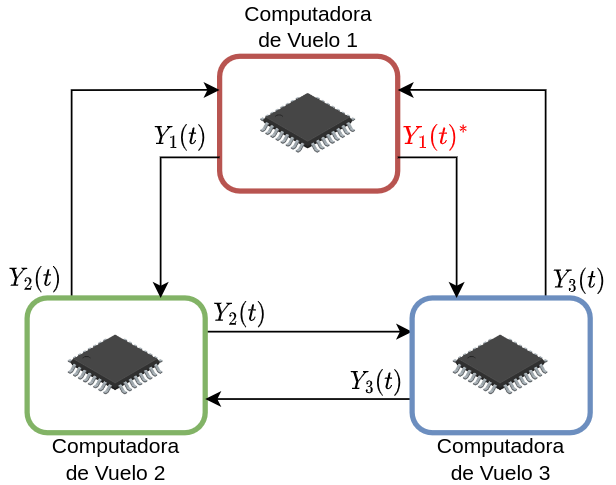
\includegraphics[width=\textwidth]{img/consenso.png}
		\column{0.5\textwidth}
			\begin{itemize}
				\item La configuración no tolera este comportamiento.
				\item Este problema se denomina: \textit{The Byzantine General's Problem.}
				\item Leslie Lamport, Rober Shostak y Marshall Pease, 1982.
				\item Se requieren $3m+1$ réplicas para tolerar $m$ ``traidores''.
			\end{itemize}
	\end{columns}
\end{frame}

\begin{frame}{Problema del Sincronismo}
	\begin{itemize}
		\item Las tareas de estimación de la pose del vehículo, y de cálculo de la señal a aplicar sobre los motores tienen requerimientos temporales fuertes.
		\item Periódicamente debe obtenerse un nuevo valor, acorde al estado en el que se encuentra el vehículo para mantenerlo estable y guiarlo.
		\item Para que las comparaciones entre réplicas tengan sentido, los resultados deben corresponder al mismo instante temporal.
		\item Esto se logra a través de una \textbf{sincronización} entre las réplicas.
	\end{itemize}
	\begin{center}
		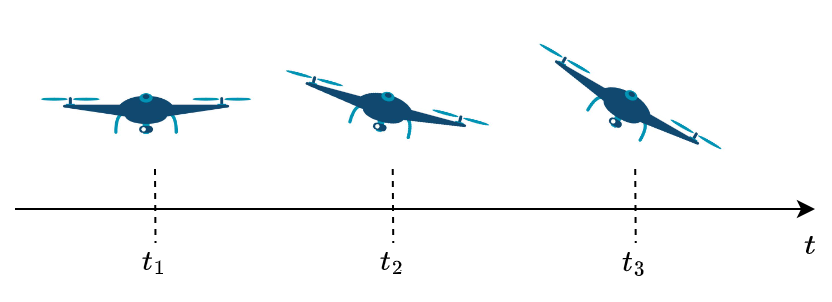
\includegraphics[width=\textwidth]{img/estados_drones.png}
	\end{center}
\end{frame}

\begin{frame}{Solución Sencilla: Bus de Comunicaciones + Sincronización}
	\begin{itemize}
		\item Una solución sencilla es utilizar un bus de comunicaciones.
		\item Cada mensaje es recibido por todas las réplicas.
		\item No hay ``traidores'.
		\item Las colisiones pueden perjudican el determinismo.
		\item Se aprovecha la sincronización para ordenar el uso del bus, acceso al medio TDMA.
		\item Esto es lo que ocurría en el caso del avión.
	\end{itemize}
	\begin{center}
		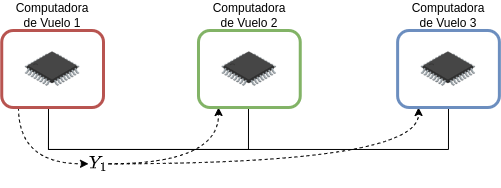
\includegraphics[width=0.8\textwidth]{img/redundancia_bus.png}
	\end{center}
\end{frame}

\begin{frame}{Requerimientos del Sistema}
	\begin{enumerate}
		\item Uso de un bus de comunicaciones.
		\item Funcionamiento sincronizado de las réplicas.
	\end{enumerate}
	\begin{columns}
		\column{0.4\textwidth}
			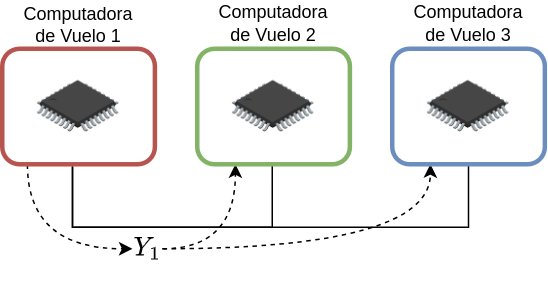
\includegraphics[width=\textwidth]{img/requerimiento_bus.png}
		\column{0.4\textwidth}
			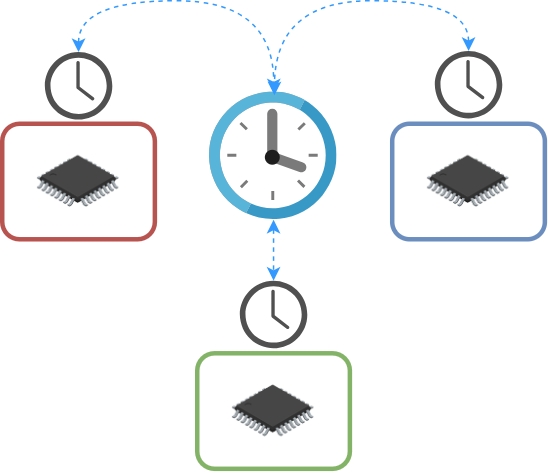
\includegraphics[width=\textwidth]{img/requerimiento_sincronismo.png}
	\end{columns}
\end{frame}